

\documentclass[11pt]{article}
\title{\textbf{Smart Classroom System Architecture Overview}}
\author{Salma El Hazal - Rim Lakhiri - Oussama Anou}
\usepackage{fullpage}
\usepackage{graphicx}

\begin{document}
	\maketitle
	The system's Block Definition Diagram is as follows:
	\begin{figure}[h]
		\begin{center}
			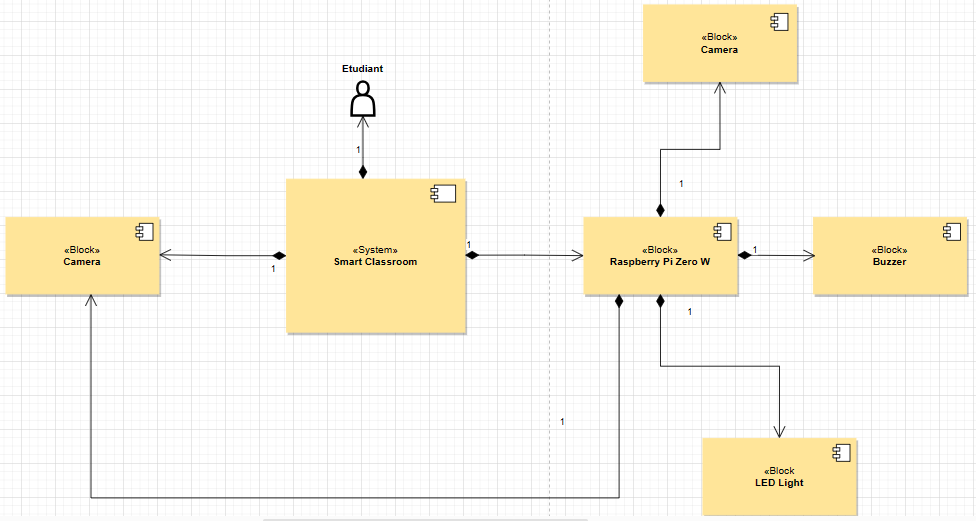
\includegraphics[width=0.7\textwidth]{SC.png}
		\end{center}
		\caption{System's BDD diagram}
	\end{figure}
	
	
	\begin{itemize}
		\item \textbf{Camera :} will be installed on the ceiling of the classroom , allows us to record and save the session.
		\item \textbf{Raspberry pi :} will be installed on  the door frame and connected to a camera in order to capture the faces and carry out the facial recognition.
		\item \textbf{Buzzer :} will be connected to the raspberry pi card and will emit sound in the case of an error such as a failed facial recognition and will emit a different sound when the facial recognition is successful.
		\item 	\textbf{LED :} the led light will also be connected to the raspberry pi card and will indicate if the facial recognition was successful or not by showing a red or green light.
		\item \textbf{Camera :} will be connected to the raspberry pi card and will. 
	\end{itemize}
	
	\pagebreak
	
	To be more specific, we decided to create a Block Definition Diagram for the Raspberry Pi:
	\begin{figure}[h]
		\begin{center}
			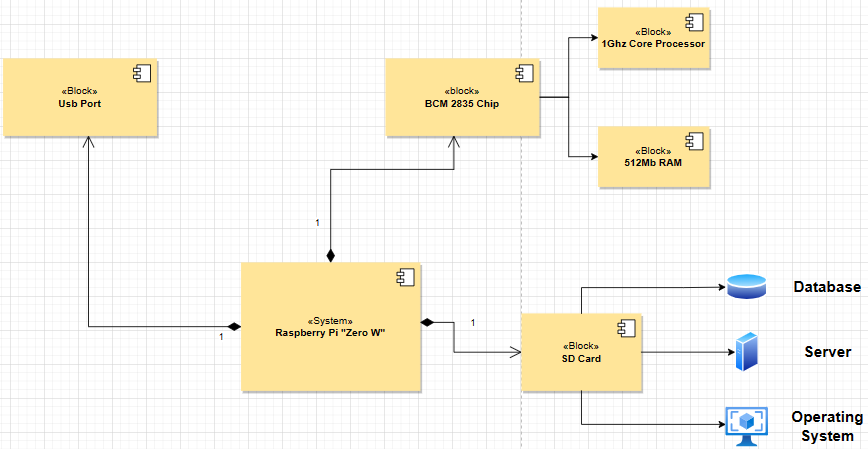
\includegraphics[width=0.7\textwidth]{RPi.png}
		\end{center}
		\caption{Raspberry's BDD diagram}
	\end{figure}
	\begin{itemize}
		\item\textbf{ USB port :} allows us to connect the card to a computer in order to code the raspberry pi.
		\item 	\textbf{Core processor :} The core processor inside a Raspberry Pi serves as the central processing unit (CPU) responsible for executing instructions and performing calculations necessary to run programs and operate the computer.
		\item \textbf{RAM :}  (Random Access Memory) in a Raspberry Pi serves as temporary storage for data that the CPU is actively using or will imminently need .
		\item \textbf{BCP chip :} specifically referring to the Broadcom BCM283x series of system-on-chip (SoC) processors, is a crucial component inside the Raspberry Pi, a popular single-board computer. This chip integrates various essential components that enable the Raspberry Pi to function as a fully-fledged computer system.
		\item \textbf{SD card :}  serves as the primary storage medium for the Raspberry Pi. It is used to store the operating system (OS), software applications, user data, and files necessary for the Raspberry Pi to function.
	\end{itemize}
	
	
	
	
\end{document}












\end{document}